

\tikzset{every picture/.style={line width=0.75pt}} %set default line width to 0.75pt        

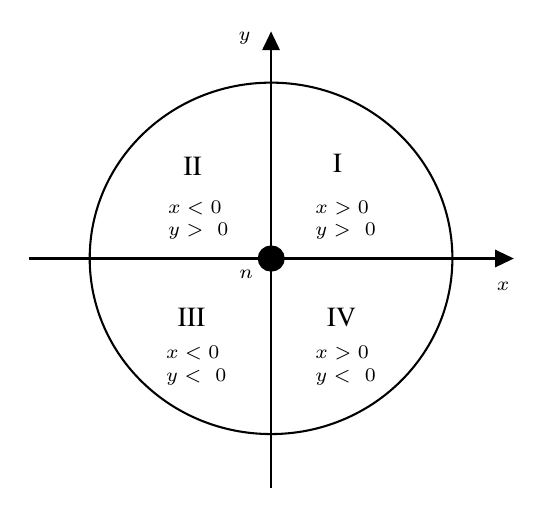
\begin{tikzpicture}[x=0.75pt,y=0.75pt,yscale=-1,xscale=1]
%uncomment if require: \path (0,300); %set diagram left start at 0, and has height of 300

%Shape: Ellipse [id:dp6073267521119902] 
\draw   (144.38,119.54) .. controls (144.38,72.78) and (183.5,34.88) .. (231.76,34.88) .. controls (280.01,34.88) and (319.13,72.78) .. (319.13,119.54) .. controls (319.13,166.29) and (280.01,204.2) .. (231.76,204.2) .. controls (183.5,204.2) and (144.38,166.29) .. (144.38,119.54) -- cycle ;
%Straight Lines [id:da17835254540908585] 
\draw    (115,119.62) -- (345.69,119.62) ;
\draw [shift={(348.69,119.62)}, rotate = 180] [fill={rgb, 255:red, 0; green, 0; blue, 0 }  ][line width=0.08]  [draw opacity=0] (8.93,-4.29) -- (0,0) -- (8.93,4.29) -- cycle    ;
%Straight Lines [id:da3214817137263065] 
\draw    (231.76,230) -- (231.76,13.24) ;
\draw [shift={(231.76,10.24)}, rotate = 90] [fill={rgb, 255:red, 0; green, 0; blue, 0 }  ][line width=0.08]  [draw opacity=0] (8.93,-4.29) -- (0,0) -- (8.93,4.29) -- cycle    ;
%Shape: Ellipse [id:dp010903733793728554] 
\draw  [fill={rgb, 255:red, 0; green, 0; blue, 0 }  ,fill opacity=1 ] (225.83,119.62) .. controls (225.83,116.4) and (228.52,113.8) .. (231.84,113.8) .. controls (235.17,113.8) and (237.86,116.4) .. (237.86,119.62) .. controls (237.86,122.84) and (235.17,125.45) .. (231.84,125.45) .. controls (228.52,125.45) and (225.83,122.84) .. (225.83,119.62) -- cycle ;

% Text Node
\draw (260,67.69) node [anchor=north west][inner sep=0.75pt]   [align=left] {{\fontfamily{ptm}\selectfont I}};
% Text Node
\draw (188.04,69) node [anchor=north west][inner sep=0.75pt]   [align=left] {{\fontfamily{ptm}\selectfont II}};
% Text Node
\draw (185.23,142) node [anchor=north west][inner sep=0.75pt]   [align=left] {{\fontfamily{ptm}\selectfont III}};
% Text Node
\draw (257.15,142) node [anchor=north west][inner sep=0.75pt]   [align=left] {{\fontfamily{ptm}\selectfont IV}};
% Text Node
\draw (214.66,8.9) node [anchor=north west][inner sep=0.75pt]  [font=\scriptsize] [align=left] {$\displaystyle y$};
% Text Node
\draw (339.06,129.44) node [anchor=north west][inner sep=0.75pt]  [font=\scriptsize] [align=left] {$\displaystyle x$};
% Text Node
\draw (245,89) node [anchor=north west][inner sep=0.75pt]  [font=\scriptsize] [align=left] {$\displaystyle  \begin{array}{{>{\displaystyle}l}}
x >0\\
y >\ 0
\end{array}$};
% Text Node
\draw (174,89) node [anchor=north west][inner sep=0.75pt]  [font=\scriptsize] [align=left] {$\displaystyle  \begin{array}{{>{\displaystyle}l}}
x< 0\\
y >\ 0
\end{array}$};
% Text Node
\draw (173,159) node [anchor=north west][inner sep=0.75pt]  [font=\scriptsize] [align=left] {$\displaystyle  \begin{array}{{>{\displaystyle}l}}
x< 0\\
y< \ 0
\end{array}$};
% Text Node
\draw (245,159) node [anchor=north west][inner sep=0.75pt]  [font=\scriptsize] [align=left] {$\displaystyle  \begin{array}{{>{\displaystyle}l}}
x >0\\
y< \ 0
\end{array}$};
% Text Node
\draw (215,123.5) node [anchor=north west][inner sep=0.75pt]  [font=\scriptsize] [align=left] {$\displaystyle n$};


\end{tikzpicture}
